\section{Arquitectura del tp2}


RELACIONAR ARQUITECTURA CON ATRIBUTOS DE CALIDAD ANTERIORES

Para empezar, se presenta la arquitectura correspondiente al Tp2.\newline

\subsection{General}

Tenemos dos formas de observar nuestra arquitectura, la primera con un enfoque general donde se ven
los componentes externos a nuestro sistema que interactúan con nosotros. Con 
esta visión, nuestra arquitectura se ve como un único componente monolítico pues es más sencillo a
este nivel, sin embargo, contamos con una arquitectura distribuida a lo largo y ancho del país 
que podremos ver con más detalle en las siguientes vistas.

\begin{figure}
\centerline{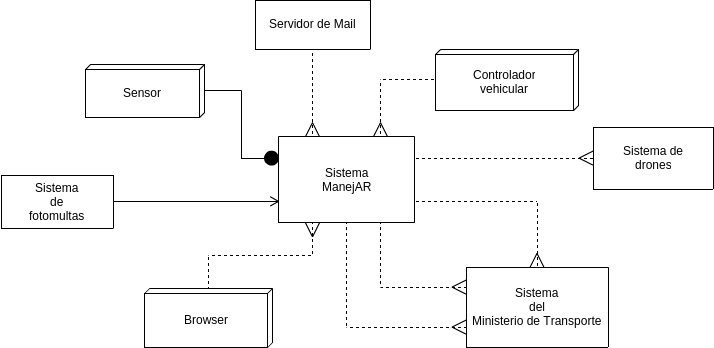
\includegraphics[width=1\textwidth]{./imagenes/arquitectura_tp2/general.png}}
\caption{Arquitectura general}
\end{figure}
%\centerline{ 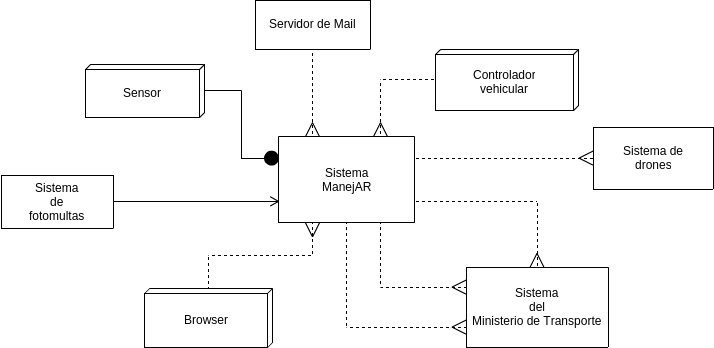
\includegraphics[width=0.7\textwidth]{./imagenes/arquitectura_tp2/general.png} } 
 % \centerline{Arquitectura general}


Como podemos ver, son varios los componentes externos que interactúan con 
nuestro sistema, cada uno con sus particularidades que pasaremos a detallar.

\subsection{Sensor}
Los \textbf{sensores} son nuestros dispositivos ubicados a lo largo del país, sobre todo en La 
Pampa, que utilizamos para medir la conectividad de la zona.
En estos dispositivos, distinguimos dos componentes claves para describir la 
arquitectura.

\begin{itemize}
  \item Receptor de mediciones de conectividad: Recolecta las mediciones del 
  hardware y las encola en el próximo componente.
  
  \item Comunicador con administrador de sensores: Toma las mediciones y las 
  envía al Administrador de sensores de nuestro sistema \textbf{ManejAR}.
\end{itemize}



La particularidad de la conexión entre este último componente y el sistema 
manejar es que el medio tiene pérdida de paquetes pero decidimos no crear una 
estrategia de reenvío pues enviamos esas mediciones cada 5 segundos.


\begin{figure}
\centerline{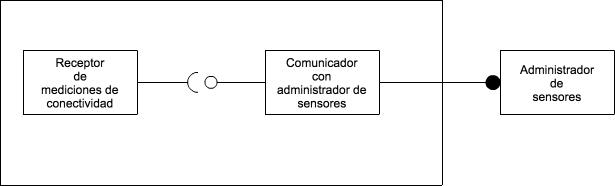
\includegraphics[width=1\textwidth]{./imagenes/arquitectura_tp2/sensor.png}}
\caption{Arquitectura interna de los Sensores}
\end{figure}

\subsection{Control Vehicular}
El controlador vehicular, es el componente que se encuentra en cada uno de los vehículos que deben
ser monitoreados. En este componente encontramos los siguientes subcomponentes.

Receptor de mediciones: Este se encarga de recibir las mediciones realizadas por el GPS de su vehículo,
 y las guarda en un repositorio de Mediciones.
 
Mediciones: Es el repositorio donde se almacenan las mediciones del GPS.
 Es importante la presencia de este componente de almacenamiento, porque nos permite preservar
las mediciones hasta el momento del envío, fundamental para no perder mediciones ante un
 problema de conectividad.
Transmitidor: Encargado de asegurarse del envio de las mediciones al Balanceador, del Sistema Manejar.
Antes de enviar cualquier dato, se comunica con el Encriptador y el Checksum para proteger la
integridad y confidencialidad de los datos. Cada medicion enviada exitosamente sera borrada del
repositorio Mediciones. En caso de no disponer de conectividad, se reintentara el envio de la medicion
cuando logre conectarse. De esta manera nos aseguramos no perder mediciones, y
 contar con todas las mediciones generadas.

\begin{figure}
\centerline{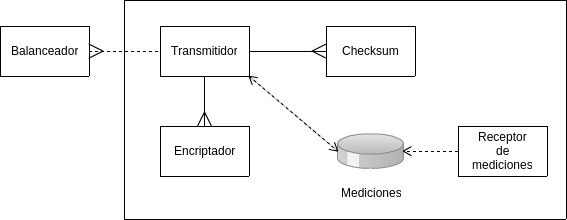
\includegraphics[width=1\textwidth]{./imagenes/arquitectura_tp2/controlador_vehicular.png}}
\caption{Arquitectura interna de los Controladores vehiculares}
\end{figure}


\subsection{Sistema Manejar}

Si nos concentramos en los componentes dentro del recuadro principal, podemos 
organizarlos en dos categorías:

* Esta en servidor central
* Distribuido en diferentes nodos a lo largo del pais.

El \textit{Controlador de datos de GPS} y el \textit{Administrador de Base de Datos} 
son los únicos que estan distribuidos en todos los nodos a lo largo del país, 
con el objetivo de optimizar el procesamiento de datos y a su vez, asegurar la 
disponibilidad del servicio ya sea del procesamiento como la redundancia de las bases de datos.


\begin{figure}
\centerline{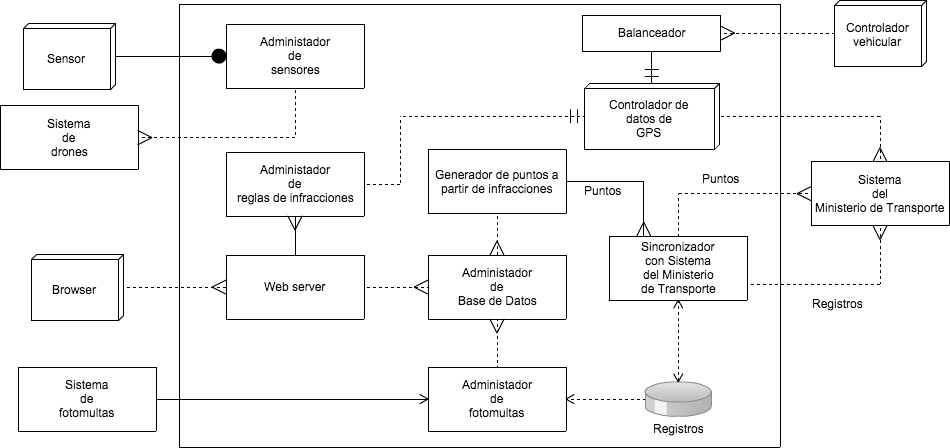
\includegraphics[width=1\textwidth]{./imagenes/arquitectura_tp2/manejar.png}}
\caption{Arquitectura interna del Sistema ManejAR}
\end{figure}

La mayoría de estos componentes los explicaremos en detalle más adelante con su 
respectiva vista. Para los que no, alcanza la siguiente descripción de los 
mismos.


\subsubsection{Administrador de reglas de infracciones}

Es el encargado de recibir las modificaciones de las reglas de infracciones y 
notificarlas a todos los \textbf{Controladores de datos de GPS} usando un \textit{broadcast}.

\subsubsection{Generador de Puntos a partir de Infracciones}

Todas las noches este componente toma las infracciones del \textbf{Administrador de Bases de Datos} 
y calcula el puntaje a restar a cada conductor. Luego se lo informa al
\textbf{Sincronizador con Sistema del Ministerio de Transporte}.

\subsubsection{Sincronizador con Sistema del Ministerio de Transporte}

Las responsabilidades de este componente son dos.
La primera es actualizar nuestra base de registros directamente del \textbf{Sistema del Ministerio de Transporte}
para poder identificar los conductores profesionales de los particulares. 
La segunda envía los puntos a descontar a cada conductor profesional.

\subsubsection{Balanceador}
El balanceo de carga es un concepto usado que se refiere a la técnica usada para compartir el trabajo
a realizar entre varios procesos, ordenadores, discos u otros recursos.
El balanceo de carga se mantiene gracias a un algoritmo que divide de la manera más equitativa posible
el trabajo, para evitar los así denominados cuellos de botella y mantener una 
alta performance y disponibilidad del sistema.


\subsection{Controlador de datos de GPS y Administrador de Bases de Datos}

\subsubsection{Controlador de datos de GPS}

Recibe las mediciones directas del GPS, las desencripta y las publica en un \textit{BUS} 
al cual estan subscriptos los siguientes componentes:

\begin{itemize}
  \item Persistidor temporal para auditoría
  \item Persistidor de datos para empresa de drones
  \item Generador de estadísticas
  \item Generador de infracciones (Múltiples instancias)
\end{itemize}

Los primeros tres son triviales, pero el último merece dar una descripción más 
detallada.

Las múltiples instancias de este proceso, comparten un mismo \textit{pipe} pero 
el primero que lo recibe lo remueve de la cola. De esta manera nos garantizamos 
que no se repita el procesamiento de los datos y poder paralelizar este 
proceso, pues la cantidad de datos en este \textit{pipe} es inmensa.
Cada una de estas instancias, deberá comunicarse con el Sistema del Ministerio 
de Transporte, para obtener los límites de velocidades. Además debe leer del 
repositorio de Reglas de infracciones, las reglas para poder generar las 
infracciones según corresponda.
Las infracciones generadas serán guardadas en un repositorio de Infracciones 
comunicándose con el \textit{Administrador de Bases de Datos}.

Las \textit{Reglas de infracciones} son actualizadas por medio de un 
\textit{ABM}, que recibe las actualizaciones del \textit{Administrador de reglas de 
infracciones}.


\subsubsection{Administrador de Bases de Datos}
Es el encargado de mantener los datos replicados en los distintos nodos, 
asegurándose de brindar una consistencia eventual entre ellos, con el objetivo 
de brindarnos performance y disponibilidad.
Es su responsabilidad, hacer de intermediario entre quienes quieran leer o 
escribir de los siguientes repositorios:

\begin{itemize}
  \item Auditoría: Guarda información para que los conductores puedan auditar 
  sus multas dentro del período de 1 mes.
  \item Estadísticas: Almacena las estadísticas generadas por el Generador de estadísticas.
  \item Drones: Guarda los datos que le seran brindados a la empresa de drones.
  \item Infracciones: Se guardan las infracciones generadas, que serán utilizadas 
  para calcular los puntajes.
\end{itemize}


\begin{figure}
\centerline{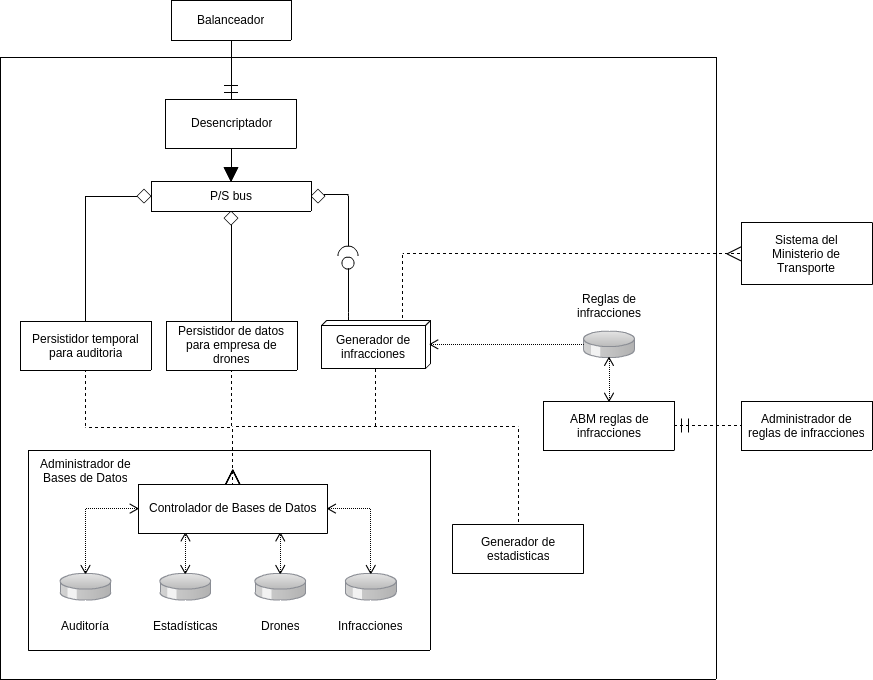
\includegraphics[width=1\textwidth]{./imagenes/arquitectura_tp2/controlador_datos_gps.png}}
\caption{Arquitectura interna del Controlador de datos de GPS del Sistema ManejAR}
\end{figure}


\subsection{Administrador de Fotomultas}
Filtra las multas recibidas del Sistema de fotomultas, para almacenar solo las 
infracciones correspondientes a conductores profesionales.
Este componente ya manda las infracciones generadas, no es necesario procesarlas,
śolo se encarga de hacer el filtro explicado anteriormente.

\begin{figure}
\centerline{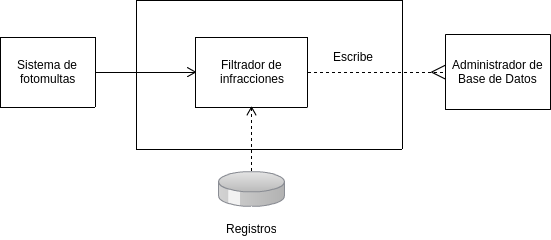
\includegraphics[width=1\textwidth]{./imagenes/arquitectura_tp2/administrador_fotomultas.png}}
\caption{Arquitectura interna del Administrador de Fotomultas del Sistema ManejAR}
\end{figure}


\subsection{Administrador de sensores}
Este proceso, es el responsable de recibir las mediciones de los sensores, que 
primero seran monitoreadas por el Monitor de sensores. Este controla que todos 
los sensores se esten comunicando periódicamente, utilizando la táctica de 
\textit{heartbeat}. En caso de no recibir mensajes de alguno de los sensores, envía una 
alerta al Comunicador con Sistema de Drones, que accionará según corresponda.
Al mismo tiempo, el Monitor de sensores, encola las mediciones al Procesador. El 
cual las almacena en un repositorio y realiza un análisis de las mediciones en 
el tiempo para detectar baja conectividad y alertar al Comunicador.
El Comunicador deberá enviar un mail a los técnicos correspondientes, al Sistema 
de drones y, además, guardar un log del uso de los drones para fines de 
auditoría.


\begin{figure}
\centerline{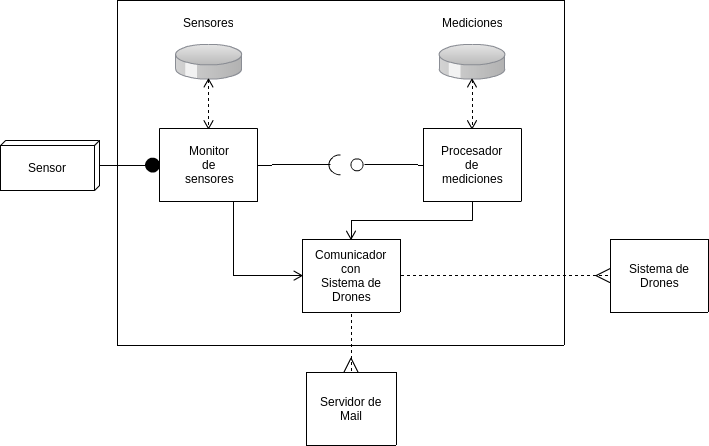
\includegraphics[width=1\textwidth]{./imagenes/arquitectura_tp2/administrador_sensores.png}}
\caption{Arquitectura interna del Administrador de Sensores del Sistema ManejAR}
\end{figure}


\subsection{Web Server}
Funciona como una interfaz, para que los distintos usuarios puedan autenticarse 
y acceder a la informacion que les corresponda segun sus permisos.


\begin{figure}
\centerline{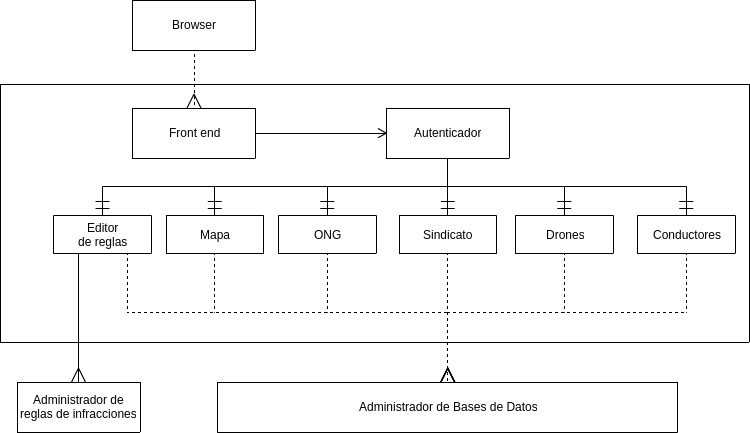
\includegraphics[width=1\textwidth]{./imagenes/arquitectura_tp2/web_server.png}}
\caption{Arquitectura interna del Web Server del Sistema ManejAR}
\end{figure}
